\subsection{Definitions and Effects}
\label{subsec:ac-basics2}

Let's dive into the fascinating world of electromagnetic waves! These waves are the backbone of radio technology, and understanding their properties is crucial. At their core, electromagnetic waves are composed of two primary components: the electric field and the magnetic field. These fields are perpendicular to each other and to the direction of wave propagation. Imagine them as two dancers moving in perfect harmony, each influencing the other. The electric field (\textbf{E}) and the magnetic field (\textbf{B}) are related by Maxwell's equations, which we can summarize as:

\begin{equation}
\nabla \times \mathbf{E} = -\frac{\partial \mathbf{B}}{\partial t}
\label{eq:maxwell1}
\end{equation}

\begin{equation}
\nabla \times \mathbf{B} = \mu_0 \mathbf{J} + \mu_0 \epsilon_0 \frac{\partial \mathbf{E}}{\partial t}
\label{eq:maxwell2}
\end{equation}

Here, $\mu_0$ is the permeability of free space, and $\epsilon_0$ is the permittivity of free space. Equations \ref{eq:maxwell1} and \ref{eq:maxwell2} show how changes in the electric field induce a magnetic field, and vice versa. This mutual induction is what allows electromagnetic waves to propagate through space.

Now, let's talk about polarization. Polarization refers to the orientation of the electric field as the wave travels. If the electric field oscillates in a single plane, the wave is said to be linearly polarized. If the electric field rotates as the wave propagates, it can be circularly or elliptically polarized. The orientation of the electric field determines the polarization state, which is crucial for applications like satellite communication and radar systems.

\begin{figure}[h]
    \centering
    % 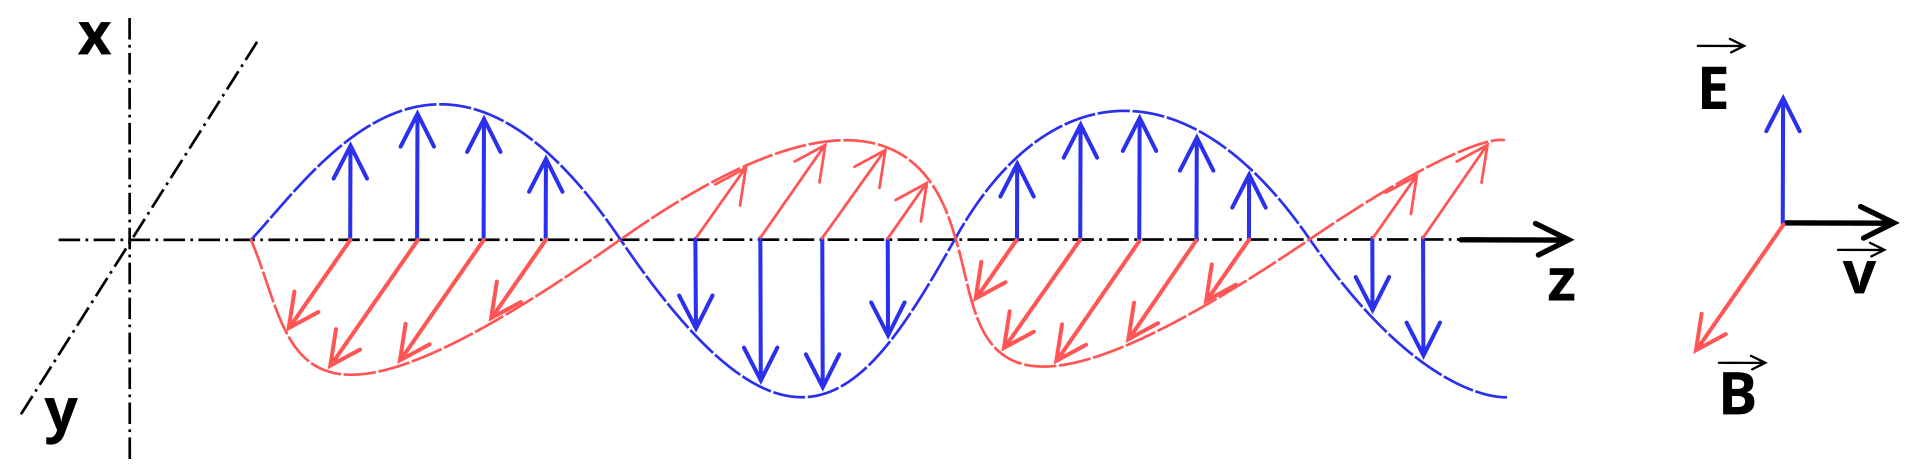
\includegraphics[width=0.8\textwidth]{em-wave.svg}
    \caption{Relationship between electric and magnetic fields in an electromagnetic wave.}
    \label{fig:em-wave}
    % Image prompt: Diagram showing the relationship between electric and magnetic fields in an electromagnetic wave. The electric field (E) and magnetic field (B) should be shown as perpendicular vectors, with the wave propagating in a direction perpendicular to both.
\end{figure}

\begin{figure}[h]
    \centering
    % 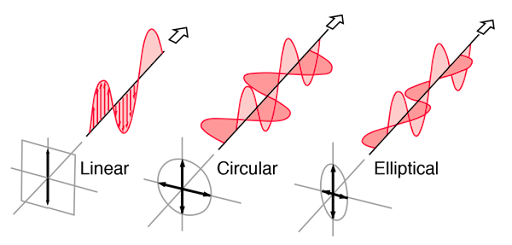
\includegraphics[width=0.8\textwidth]{polarization.svg}
    \caption{Radio wave polarization determined by the orientation of the electric field.}
    \label{fig:polarization}
    % Image prompt: Illustration of radio wave polarization showing the orientation of the electric field. The electric field should be shown oscillating in different planes for linear, circular, and elliptical polarization.
\end{figure}

In summary, the electric and magnetic fields are the yin and yang of electromagnetic waves. They work together to create the waves that carry information across vast distances. Understanding their relationship and the concept of polarization is essential for anyone working in radio technology. So, next time you tune into your favorite radio station, remember the intricate dance of electric and magnetic fields that makes it all possible!
